\chapter{Widest paths}%
\label{chap:08}

\setcounter{section}{1}
\section{Shortest vs.\ widest paths}
In the ``classical'' shortest path algorithms discussed so far the
length of a path was given by the \textbf{sum} of the edge weights. In
this chapter we discuss widest path (bottleneck shortest path/ maximum
capacity path/ minimax path) methods.  Here, the length of a path is
given by the \textbf{single largest} (smallest) edge weight.
\todo{1D example from lecture}

\section{Minimax paths and Prim's algorithm}
Recall Disjkstra's Algorithm from a previous lecture. At each
iteration we do the following: take the node $v$ from the list of
nodes that have not yet been visited with the smallest distance from
the starting node. Denote by $e = (v,u)$ the edge from $v$ to $u$.  In
the ``classical'' Dijkstra algorithm (where we want to compute the
shortest path from the starting vertex to each of the other nodes) we
now do the following: For each edge $e(v,u)$, $u$ in the forward-star
(\ie the set of edges connecting ``outgoing'' nodes) of $v$, update
the distance to the node $u$ according to
\begin{equation*}
  d(u) = \min\{d(u), d(v) + w(e) \}\,,
\end{equation*}
where $w(e)$ is the edge weight of $e$. If we want to compute the
minimax path, we can still use the same idea; however, we instead
update $d(u)$ by
\begin{equation*}
  d(u) = \min\{d(u), \max\{ d(v), w(e) \}\}\,,
\end{equation*}
since we are only interested in the single most expensive edge on the
way from the starting node to $u$. This change essentially leads to a
related algorithm, called (eager) Prim's algorithm. Instead of finding
the shortest path we now build a spanning tree, \ie a minimal tree
that contains every node of the graph. We see that the shortest path
problem and the minimax problem are in essence the same problem only
with different definition of what we mean by the distance between two
nodes. In other words: both a shortest path problems with a different
notion of what it means to be short. Algebraic graph theory, which is
discussed in the next chapter, provides a unified framework to better
understand this relationship.

\section{All-pairs minimax paths and the minimum spanning tree}
A minimum spanning tree (MST) is a subgraph with the shape of a tree (\ie it
contains no loops) that is spanning (\ie each node can be reached from any other
in the subgraph) whose sum of edge weights is minimal. Every edge not in the MST
is at least as large/ heavy/ costly as all other edges in the loop induced by
adding that edge to a MST (``cycle property''), see Figure~\ref{fig:mst}.
\begin{figure}[htpb]
  \centering 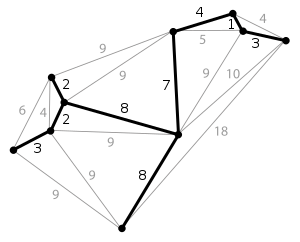
\includegraphics[width=0.6\textwidth]{Figures/MST}
  \caption{A minimum spanning tree.}%
  \label{fig:mst}
\end{figure}

It turns out that the path from some node $u$ to some other node $v$ in the MST
of an undirected graph is a minimax path between $u$ and $v$ in that graph. The
converse is not true in general: the union of the minimax paths between all
nodes is not necessarily a tree and hence in particular it need not be the MST.

Further, in an undirected graph with non-negative edge weights, the minimax
distance between pairs of vertices defines an \textbf{ultrametric}.

\begin{definition*}
  An ultrametric $d_{uv}$ is a metric with the following additional property
  \begin{equation*}
    d_{uv} \le \max\{ d_{uw}, d_{wv}\}\,,
  \end{equation*}
  the so called \emph{strong triangle inequality} (or ultrametric inequality).
\end{definition*}
Note that the ultrametric inequality implies that there exists a permutation
$(i,j,k)$ of three vertices $(u,v,w)$ such that
\begin{equation*}
  d_{ij} \le d_{ik} = d_{kj}\,.
\end{equation*}
This, in trurn, implies that a set of points in an ultrametric space can always
be represented as leaves in a binary rooted tree that all have the same distance
from the root (a so called \emph{ultramteric tree}). Consider again the MST from
Figure~\ref{fig:mst}. We can build the corresponding ultrametric tree as
follows. Start with the nodes that have the smallest distance, draw them as
leaves of a tree and connect them to the same parent that is located at the
``height'' that corresponds to their distance (see Figure below; we start with
the two nodes on the top right that are connected by an edge with weight
one). Then we take the node that is next closest and connect the subtree from
the previous step to this node (in the Figure~\ref{fig:ultramteric:tree}, now
all vertices within the green ellipse are processed). We then repeat this
process until no more nodes are left. The ultrametric distance between two nodes
is then given by the height of their least common ancestor in the ultrametric
tree. Note that there exist data structures such that finding the least common
ancestor of two nodes is an $\mathcal{O}(1)$ operation.

\begin{figure}[htpb]
  \centering
  \begin{subfigure}[c]{0.4\textwidth}
    \begin{tikzpicture}
      \node[anchor=south west,inner sep=0] at (0,0)
      {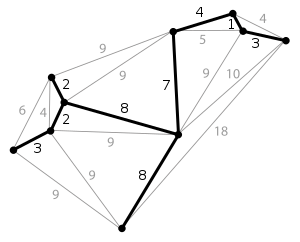
\includegraphics[width=\textwidth]{Figures/MST}};

      \draw[red, rotate around={-60:(5.15,4.7)}] (5.15,4.7) ellipse (0.4cm and
      0.2cm); \draw[green, rotate around={-120:(5.6,4.5)}] (5.6,4.5) ellipse
      (0.5cm and 1cm); \draw[blue, rotate around={0:(5,4.55)}] (5,4.55) ellipse
      (1.5cm and 0.5cm); \draw[cyan, rotate around={0:(4.5,3.7)}] (4.5,3.7)
      ellipse (2cm and 1.6cm); \draw[magenta, rotate around={0:(0,0)}] (1.2,3)
      ellipse (0.3cm and 0.8cm); \draw[olive, rotate around={-40:(0.9,2.9)}]
      (0.9,2.8) ellipse (0.7cm and 1.2cm); \draw[violet, rotate
      around={-50:(3,2.9)}] (3.1,2.9) ellipse (2.1cm and 4cm);
    \end{tikzpicture}
  \end{subfigure}
  \begin{subfigure}[c]{0.4\textwidth}
    \includegraphics[width=\textwidth]{Figures/ultrametric_tree.tikz}
  \end{subfigure}
  \caption{Minimum spanning tree and corresponding ultrametric tree. The
    ultrametric tree is built by repeatedly finding the nodes that have the
    smallest distance to the nodes already processed (indicated by the
    ellipses).}%
  \label{fig:ultramteric:tree}
\end{figure}

\section{Seeded watershed segmenation}
\todo{Finish lecture}
\section{Learned watershed}
\todo{Finish lecture}



% (again, the distance between two nodes can be defined as the sum of
% all intermediate edges or the maximum edge leading to a shortest
% path problem and a minimax problem, respectively). This can be
% achieved with a very similar algorithm which is called Prim's
% algorithm. In a minimum spanning tree the \textbf{total} cost of all
% edges is minimial along all trees that contain every node of the
% graph. This does \textbf{not} guarantee that the path between two
% nodes is the smallest possible within the graph.
%%% Local Variables:
%%% mode: latex
%%% TeX-master: "../main"
%%% End:
